\documentclass[10pt]{article} % Font size - 10pt, 11pt or 12pt

\usepackage[hmargin=1.25cm, vmargin=1.5cm]{geometry} % Document margins

\usepackage[usenames,dvipsnames]{xcolor} % Allows the definition of hex colors

% Fonts and tweaks for XeLaTeX
\usepackage{fontspec,xltxtra,xunicode}
\defaultfontfeatures{Mapping=tex-text}
%\setmonofont[Scale=MatchLowercase]{Andale Mono}

% Colors for links, text and headings
\usepackage{hyperref}
\definecolor{linkcolor}{HTML}{506266} % Blue-gray color for links
\definecolor{shade}{HTML}{F5DD9D} % Peach color for the contact information box
\definecolor{text1}{HTML}{2b2b2b} % Main document font color, off-black
\definecolor{headings}{HTML}{701112} % Dark red color for headings
% Other color palettes: shade=B9D7D9 and linkcolor=A40000; shade=D4D7FE and linkcolor=FF0080

\hypersetup{colorlinks,breaklinks, urlcolor=linkcolor, linkcolor=linkcolor} % Set up links and colors

\usepackage{fancyhdr}
\usepackage{amsmath}
\usepackage{amssymb}
\usepackage{verbatim}
\pagestyle{fancy}
\fancyhf{}

\renewcommand{\headrulewidth}{0pt} % Get rid of the default rule in the header

\usepackage{titlesec} % Allows creating custom \section's

% Format of the section titles
\titleformat{\section}{\color{headings}
\scshape\Large\raggedright}{}{0em}{}[\color{black}\titlerule]

\title{Dynein project log}
\author{Elliott Capek}
\titlespacing{\section}{0pt}{0pt}{5pt} % Spacing around titles

\begin{document}

\maketitle{}

\section{Equipartition Theorem}
The Equipartition Theorem (ET) predicts the average energy per degree of freedom of a system with energy which depends on the square of each degree of freedom. Mathematically is is expressed as:

\begin{align*}
  Z &= \int_{-\infty}^{\infty} e^{-\beta Ax^2}dx = \sqrt{\frac{\pi}{\beta A}}\\
  <E> &= - \frac{d\ln Z}{d\beta} = -\left(\sqrt{\frac{\beta A}{\pi}}\right)\left(\frac{\sqrt{\beta A}}{2\sqrt{\pi}}\right)\frac{-\pi}{A\beta^2}\\
  &= \frac{1}{2}k_BT\\
\end{align*}

where Z is the partition function and x a degree of freedom.\\

For our model, each domain feels three separate forces:

\textbf{Brownian forces}: Random forces due to water particle collisions. Gaussian-sampled with a
variance $\sqrt{\frac{\gamma k_BT}{dt}}$. Brownian forces are somehow necessary for the ET energy
to be realized.\\

\textbf{Conformational forces}: Spring forces from the molecule deviating from its lowest-energy
conformation. The energy from these forces is quadratic with respect to angle, and so each free
angle should contribute to the average energy by ET.\\

\textbf{Internal forces}. Tension forces (constraint forces) felt between domains which keep
the protein rigid. These are not quadratic, so it is unclear how they contribute to energy!\\

\subsection{Onebound case}
The conformational forces are:\\
\begin{align*}
  |\vec{F_{ub}}| &\approx \frac{c_m\theta_{um}}{L_s}\\
  |\vec{F_{um}}| &\approx \frac{c_m\theta_{um}}{L_s} + \frac{c_m\theta_{um}}{L_t} + \frac{c_t\theta_{t}}{L_t}\\
  |\vec{F_{t}}| &\approx \frac{c_m\theta_{um}}{L_t} + 2\frac{c_t\theta_t}{L_t} + \frac{c_m\theta_{bm}}{L_t}\\
  |\vec{F_{bm}}| &\approx \frac{c_t\theta_t}{L_t} + \frac{c_m\theta_{bm}}{L_t} + \frac{c_m\theta_{bm}}{L_s} + \frac{c_b\theta_{bb}}{L_s}\\
  |\vec{F_{bb}}| &\approx \frac{c_m\theta_{bm}}{L_s} + \frac{c_b\theta_{bb}}{L_s}\\
\end{align*}

From this we can come up with rough order-of-magnitude estimates of the energy of each domain is:

\begin{align*}
  PE_{ub} &\approx \frac{c_m}{L_s}\theta_{um}^2 + \frac{c_m}{L_t}\theta_{um}^2\\
  PE_{t} &\approx \frac{c_t}{L_t}\theta_{t}^2\\
  PE_{bm} &\approx \frac{c_m}{L_s}\theta_{bm}^2 + \frac{c_m}{L_t}\theta_{bm}^2\\
  PE_{bb} &\approx \frac{c_m}{L_s}\theta_{um}^2\\
\end{align*}

From this we can see that the conformational PE of each domain depends on different combinations of
stalk/tail length and spring constants.

\textbf{When is equipartition behaved?}
It seems like ET should be behaved when we have an even balance of Brownian and conformational forces:

\begin{align*}
  F_{conf} &\approx F_{Brownian}\\
  \frac{c}{L}\theta &\approx \sqrt{\frac{k_BT\gamma}{dt}}\\
\end{align*}

Is this reflected in our simulation? Well take a look at %% Fig ($\ref{fig:latent-heat}$)
...

%% \begin{figure}[h!]
%%   \centering
%%   \includegraphics[width=0.5\textwidth]{../figures/ob_equipartition_vs_force_ratio.pdf}
%%   \caption{Onebound conformational energy follows equipartition best when the ratio of conformational
%%   forces to Brownian forces is one.}
%%   \label{fig:equipartition_vs_force_ratio}
%% \end{figure}

\section{Brownian motion}
\subsection{Derivation} \label{sec:bmotion-derivation}
We can derive the equation for the position of a particle using the simple Newtonian mechanics. We
start with the general $2^{nd}$ law equation for a particle with random forces and drag (the
Langevin equation). We then take the time-averages of all variables (using expectation value signs)
to eliminate the effect of random Brownian forces. After some algebra we arrive at a differential
equation for squared position. We solve it and simplify its expression for limits when $t >> \tau$
and $t << \tau$.\\

\begin{align*}
  \frac{d\vec{v}}{dt} &= \frac{1}{m}\left(\frac{-mv}{\tau} + R\right)\\
  \frac{d\vec{v}}{dt} &= \frac{-v}{\tau} + \frac{R}{m}\\
  <\vec{r} \cdot \frac{d\vec{v}}{dt} > &+ \frac{1}{\tau}<\vec{r} \cdot \vec{v}> = 0\\
  \frac{1}{2}\frac{d^2}{dt^2}(r^2) &+ \frac{1}{2\tau}\frac{d}{dt}(r^2) - v^2 = 0 \hspace{1cm} \Bigg(\mbox{b/c }\frac{d}{dt}\left(\vec{r} \cdot \vec{v}\right) = v^2 + \left(\vec{r} \cdot \frac{d\vec{v}}{dt}\right)
  \mbox{ and }
  \frac{d}{dt}\left(\vec{r} \cdot \vec{r}\right) = 2\left(\vec{r} \cdot \vec{v}\right) \Bigg)\\
  \frac{d^2}{dt^2}(<r^2>) + &\frac{1}{\tau}\frac{d}{dt}(<r^2>) = 2<v^2> = \frac{6k_BT}{m} \hspace{1cm}\left(\mbox{Equipartition Theorem}\right)\\
  <r^2> &= \frac{6k_BT\tau^2}{m}\left(e^{-t/\tau}-1+\frac{t}{\tau}\right)\\
\end{align*}

so...

\begin{align*}
  \left(t << \tau \right) \rightarrow <r^2> = \frac{3k_BT}{m}t^2 \hspace{2cm}\mbox{free particle motion}\\
  \left(t >> \tau \right) \rightarrow <r^2> = \frac{6k_BT\tau}{m}t \hspace{2cm}\mbox{motion proportional to }\sqrt{t}\\
\end{align*}

\textbf{Averaging over time?}
In the above derivation we use time averaging to eliminate the effect of Brownian forces. This is
essentially just discussing the motion of a particle on a timescale where Brownian forces go to
zero. The variance of the Brownian force R is:

\begin{align*}
  \sigma_R^2 &= \sqrt{\frac{2k_BTm}{\tau dt}}\\
\end{align*}

(TODO: further justify the dt in the variance)\\
Thus over larger timescales (bigger dt's) the Brownian force is smaller. When time averaging, all
we are saying is that our dt is large enough that Brownian forces are negligible.\\

An interesting observation is that the motion equation for a particle feeling Brownian forces is
identical to the equation for a macroscopic object feeling drag forces, which makes sense, since
to solve the Brownian motion equation we just eliminate R.\\

\section{Brownian dynamics}
We use Brownian dynamics as our equation of motion. BD is just the special case of Langevin dynamics

\begin{align*}
  m\frac{d\vec{v}}{dt} &= -\frac{m}{\tau}\vec{v} + \vec{F} + \vec{R}\\
\end{align*}

where $m\rightarrow0$:

\begin{align*}
  \vec{v} &= \frac{\tau}{m}\vec{F} + \frac{\tau}{m}\vec{R}\\
\end{align*}

where m is the mass, $\tau$ the time constant, $\vec{F}$ a generic force and $\vec{R}$ the Brownian
force. Mass ``going to zero'' means we are discussing particles where $m << $ any other variable.
Because m is tiny the particle effectively has no net force on it, so the drag force must cancel
out the other forces. From this we can find velocity.\\

\subsection{What is $\tau$?}
Tau is a time constant that describes the behavior of a system with respect to time. By looking at
the motion equations for Brownian systems in Section (\ref{sec:bmotion-derivation}), we see that the
size of t with respect to $\tau$ decides what type of motion the particle will feel. On the ``small''
timescale the system displays free particle motion, but on the ``large'' timescale, the system
displays Brownian motion. $\tau$ can be thought of as the time the system switches from free to
Brownian motion.\\

\section{Finding a reasonable dt}
TODO: describe the relationship between diffusion constant D, time constant $\tau$ and dt.\\

\subsection{Relating D to $\tau$}

I don't really understand this derivation:

\begin{align*}
  \sin\left(\Delta\theta\right) &\approx \Delta\theta = \frac{x}{L}\\
  \Delta\theta^2 &= \frac{x^2}{L^2} = \frac{Dt}{L^2}\\
\end{align*}

We set our $\tau$ to be the time when $<\Delta\theta^2> \approx 1$, so:

\begin{align*}
  \tau = \frac{L^2}{D}\\
\end{align*}

\subsection{Finding D}
For a particle feeling Brownian forces:

\begin{align*}
  \frac{\Delta x}{\Delta t} &= \frac{\tau}{m} R\\
\end{align*}

We say the magnitude of R is the standard deviation of a Gaussian process:

\begin{align*}
  \frac{\Delta x}{\Delta t} &= \frac{\tau}{m}\sqrt{\frac{2k_BTm}{\tau \Delta t}}\\
  \Delta x &= \sqrt{\frac{2k_BT\tau}{m\Delta t}}\Delta t\\
  <\Delta x^2> &= \frac{2k_BT\tau}{m}\Delta t\\
\end{align*}

We then use the Brownian motion equation for $t >> \tau$ to find D:\\

\begin{align*}
  <\Delta x^2> &= D\Delta t = \frac{2k_BT\tau}{m}\Delta t\\
  D = \frac{2k_BT\tau}{m} = \frac{2k_BT}{\gamma}\\
\end{align*}

\subsection{Alternative derivation of D (Einstein relation)}
We can also arrive at an expression for D through an equilibrium argument. There are two forces which cause currents in solutions: drift and diffusion.
Drift is motion due to a force acting on particles. Diffusion is current due to random, natural motions of particles. Our equilibrium condition is when
the flux of particles due to both effects is equal, so there is no net particle flow. We first need to describe these fluxes:\\

\textbf{Drift flux}\\
Our particles obey Brownian dynamics, so $\gamma\dot{x} = F$, where $\gamma$ is the drag force constant. Flux J, or particles per second-area, can be
found by multiplying the velocity of particles by the concentration $\rho$:

\begin{align*}
  J_{drift} &= \frac{1}{\gamma}F(x)\rho(x)\\
  &= -\frac{1}{\gamma}\rho(x)\nabla U\\
\end{align*}

\textbf{Diffusion flux}\\
Flux due to diffusion is proportional to the negative gradient in concentration and D:

\begin{align*}
  J_{diff} &= -D\nabla \rho(x)\\
\end{align*}

\textbf{Solving for D}\\
The concentration gradient in a solution is proportional to the energy gradient. By the chain rule:

\begin{align*}
  \nabla \rho &= \frac{\partial\rho}{\partial U} \nabla U\\
\end{align*}

We then set the sum of our two fluxes to zero and solve for the equilibrium condition:

\begin{align*}
  J_{diff} + J_{drift} &= 0\\
  -\frac{1}{\gamma}\rho(x)\nabla U - D\nabla \rho(x) &= 0\\
  \frac{1}{\gamma}\rho(x)\nabla U + D \frac{\partial\rho}{\partial U} \nabla U&= 0\\
  \left(\frac{1}{\gamma}\rho(x) + D\frac{\partial\rho}{\partial U}\right)\nabla U &= 0\\
\end{align*}

because $\nabla U$ is not guarenteed to be zero everywhere, it must be the case that:

\begin{align*}
  \frac{1}{\gamma}\rho(x) &= -D\frac{\partial\rho}{\partial U}\\
  \frac{-\rho(x)}{\gamma\frac{\partial\rho}{\partial U}} &= D\\
\end{align*}

\textbf{Finding d$\rho$/dU}\\
To simplify this value, we note that, because the particles do not interact, energy is purely a function of position. Thus, by
Maxwell-Boltzman statistics, the probability of being at a location x (i.e $\rho(x)$) is proportional to $e^{-\beta U(x)}$.
From this we can find an expression for concentration and d$\rho(x)/dU(x)$:

\begin{align*}
  \rho(x) &= Ae^{-\beta U(x)}\\
  \frac{\partial \rho(x)}{\partial U} &= \frac{-1}{k_BT}Ae^{-\beta U(x)}\\
\end{align*}

Plugging these expressions into our D equation, in addition to our definition for $\gamma$, we can see that:

\begin{align*}
  \frac{-1}{\gamma\frac{-1}{k_BT}} &= D\\
  D &= \frac{k_BT}{\gamma} = \frac{k_BT\tau}{m}\\
\end{align*}

\section{Equipartition Theorem for quadratic energies}
\begin{align*}
  Z &= \int_{-\infty}^{\infty} e^{-\beta Ax^2}dx = \sqrt{\frac{\pi}{\beta A}}\\
  <E> &= - \frac{d\ln Z}{d\beta} = -\left(\sqrt{\frac{\beta A}{\pi}}\right)\left(\frac{\sqrt{\beta A}}{2\sqrt{\pi}}\right)\frac{-\pi}{A\beta^2}\\
  &= \frac{k_BT}{2}\\
\end{align*}

\section{Gamma derivation}

Stoke's Law states that the relationship between viscosity, force, and
velocity for a spherical particle is given by:
\begin{align}
  \mathbf{v} &= \frac{\mathbf{F}}{6\pi \mu R}
\end{align}
where $\mu$ is the viscosity of the fluid, and $R$ is the radius of
the particle.  Thus in our terminology:
\begin{align}
  \gamma &= 6\pi \mu R.
\end{align}
Note that the viscosity of water is temperature-dependent and around
0.7~mPa~s at body temperature.  However, the viscosity of cytoplasm
may be rather different, and will of course depend on length scale.
But for our purposes we can probably get away with this value.

The random force $\mathbf{R}(t)$ should have a Gaussian distribution
with variance~1, but then be divided by $\sqrt{\Delta t}$.  Thus, the
smaller the time step, the larger the random force we will apply.  We
can understand this in the backwards direction.  When we observe a
larger time step, the ``random force'' results from many smaller
random forces added together, and these smaller forces often cancel,
leading to this reduction in the total force over that time period.

Finally, we will need estimates for the radii of each domain (to go
into the $\gamma$ parameter, the equilibrium angles for each hinge, and
the spring constants for each hinge.  The first two we can estimate
from the structure of dynein.  The third will require a rough guess.
We can get a ball-park guess by deciding how much we want the angle to
fluctuate (e.g. $\ll \pi$ for each angle!), and then take our spring
constant to be $kT$ divided by that anglular fluctuation squared.

\section{Background of Correlation function}
This is based on the Autocorrelation procedure (see Convolution on Wikipedia).
In our correlation function code, we take the autocorrelation function of our
potential and time-translate it to get the time at which there is zero correlation
between the functions. Flesh this out sometime!\\

\section{CLT (and/or Brownian distribution is Gaussian?) Derivation}
Here we show that, given an initial PDF as a delta function $P(t_0,x) = \delta(x)$
and any transition likelihood $W(s)$ for some step size s and 1 timestep, P
eventually evolves into a Gaussian function.\\

We use a discrete time, continuous position model:\\

\begin{align}
  P(t_0+1,x') &= \int_{-\infty}^{\infty}W(x'-x)P(t_0,x)dx
\end{align}

This matches the form of a convolution integral:

\begin{align*}
  (P*W)(x') &= \int_{-\infty}^{\infty}P(t_0,x)W(x'-x)dx
\end{align*}

By the Convolution Theorem (prove?) we can simplify the above expression:

\begin{align}
  F\{P(t_0+1,x')\} &= F\left\{\int_{-\infty}^{\infty}W(x'-x)P(t_0,x)dx\right\}\\
  \widetilde{P}(t_0+1,k) &= \widetilde{W}(k)\widetilde{P}(t_0,k)
\end{align}

We now let our initial time $t_0$ be zero and note that, because
$W_n(\Delta x) = W(\Delta x)^n$, we can simplify our expression to:

\begin{align}
  \widetilde{P}(n,k) &= \widetilde{W}(k)^n\widetilde{P}(t_0,k)
\end{align}

We then take the Inverse Fourier Transform of this expression, yielding:

\begin{align}
  P(n,x) &= \int_{-\infty}^{\infty}\widetilde{P}(n,k)e^{2\pi ikx}dk
  = \int_{-\infty}^{\infty}\widetilde{W}(k)^n\widetilde{P}(t_0,k)e^{2\pi ikx}dk
\end{align}

Since $P(0,x)$ is a delta function, we know that $\widetilde{P}(0,x) = 1$, so:

\begin{align}
  P(n,x) &=  \int_{-\infty}^{\infty}\widetilde{W}(k)^ne^{2\pi ikx}dk
\end{align}

The Taylor Series for $\widetilde{W}(k)$ is:

\begin{align*}
  \widetilde{W}(k) &= \widetilde{W}(0) + k\widetilde{W_1}(0) + \frac{k^2}{2}\widetilde{W_2}(0) + \frac{k^3}{6}\widetilde{W_3}(0) + ...\\
  &= 1 + k\widetilde{W_1}(0) + \frac{k^2}{2}\widetilde{W_2}(0) + \frac{k^3}{6}\widetilde{W_3}(0) ...\\
\end{align*}

We define a variable $\widetilde{W}$ such that:

\begin{align*}
  \widetilde{W}(k) &= 1 - \widetilde{C}\\
  \widetilde{C} &= -(k\widetilde{W_1}(0) + \frac{k^2}{2}\widetilde{W_2}(0) + \frac{k^3}{6}\widetilde{W_3}(0) ...)\\
\end{align*}

This allows us to substitute in $\widetilde{C}$ and use the Binomial Expansion:

\begin{align}
  P(n,x) &=  \int_{-\infty}^{\infty}\left(1 - \widetilde{C}\right)^ne^{2\pi ikx}dk\\
  &= \int_{-\infty}^{\infty}\left(\sum_{\alpha=0}^n {}_nC_\alpha\left(-\widetilde{C}\right)^\alpha\right)e^{2\pi ikx}dk\\
  &= \int_{-\infty}^{\infty}\left(\sum_{\alpha=0}^n \frac{n!(-1)^\alpha}{(n-\alpha)!\alpha!} \widetilde{C}^\alpha\right)e^{2\pi ikx}dk
\end{align}

The Taylor Series of our goal, the Gaussian function, is:\\

\begin{align*}
  e^{\frac{-x^2}{2\sigma^2}} &= \sum_{\alpha=0}^\infty \frac{(-1)^\alpha}{\alpha!}\left(\frac{x}{\sqrt{2}\sigma}\right)^{2\alpha}
\end{align*}

We want to make our expression for $P(n,x)$ resemble this. We begin by saying that, for sufficiently large $n$, the higher-order
$\alpha$ terms in the sum go to zero due to the $1/\alpha!$. Thus, we can extend our sum to infinity:\\

\begin{align}
  P(n,x) &= \int_{-\infty}^{\infty}\left(\sum_{\alpha=0}^\infty \frac{(-1)^\alpha}{\alpha!}\frac{n!}{(n-\alpha)!} \widetilde{C}^\alpha\right)e^{2\pi ikx}dk
\end{align}

We then apply Sterling's Approximation in the form $Z! = e^{Z\ln(Z)-Z}$:

\begin{align}
  P(n,x) &= \int_{-\infty}^{\infty}\left(\sum_{\alpha=0}^\infty \frac{(-1)^\alpha}{\alpha!}\frac{e^{n\ln(n)-n}}{e^{(n-\alpha)\ln(n-\alpha)-(n-\alpha)}} \widetilde{C}^\alpha\right)e^{2\pi ikx}dk\\
  &= \int_{-\infty}^{\infty}\left(\sum_{\alpha=0}^\infty \frac{(-1)^\alpha}{\alpha!}\frac{n^ne^{-n}}{(n-\alpha)^{n-\alpha}e^{\alpha-n}} \widetilde{C}^\alpha\right)e^{2\pi ikx}dk
\end{align}

Because n is large, we can get rid of its decaying exponentials and simplify:\\

\begin{align}
  P(n,x) &= \int_{-\infty}^{\infty}\left(\sum_{\alpha=0}^\infty \frac{(-1)^\alpha}{\alpha!}\frac{n^n}{(n-\alpha)^{n-\alpha}e^{\alpha}} \widetilde{C}^\alpha\right)e^{2\pi ikx}dk\\
  &= \int_{-\infty}^{\infty}\left(\sum_{\alpha=0}^\infty \frac{(-1)^\alpha}{\alpha!}\frac{n^n}{(n-\alpha)^{n-\alpha}} \sqrt{\frac{\widetilde{C}}{e}}^{2\alpha}\right)e^{2\pi ikx}dk\\
  &= \int_{-\infty}^{\infty}\left(\sum_{\alpha=0}^\infty \frac{(-1)^\alpha}{\alpha!}\frac{n^\alpha}{(1-\frac{\alpha}{n})^{n-\alpha}} \sqrt{\frac{\widetilde{C}}{e}}^{2\alpha}\right)e^{2\pi ikx}dk
\end{align}

%% We now use the following simplification, assuming that $\alpha/n < 1$:

%% \begin{align*}
%%   \left(1-\frac{\alpha}{n}\right)^{n-\alpha} &= \sum_{x=0}^{n-\alpha} \frac{(n-\alpha)!}{(n-\alpha-x)!x!} \left(\frac{\alpha}{n}\right)^x\\
%%   &= 1 - (n-\alpha)\left(\frac{\alpha}{n}\right) + (n-\alpha)(n-\alpha-1)\left(\frac{\alpha}{n}\right)^2\\
%%   &= 1 - \alpha + \frac{\alpha^2}{n} + \alpha^2 + \frac{-\alpha^3}{n} + \frac{-\alpha^2}{n} + \frac{-\alpha^3}{n} + \frac{\alpha^4}{n^2} + \frac{\alpha^3}{n^2}\\
%%   &= 1 - \alpha + \alpha^2 + \frac{-2\alpha^3}{n} + \frac{\alpha^4}{n^2} + \frac{\alpha^3}{n^2}\\
%% \end{align*}

We then supply the middle factorial fraction with a name, $m = \frac{1}{(1-\frac{\alpha}{n})^{n-\alpha}}$:

\begin{align}
  P(n,x) &= \int_{-\infty}^{\infty}\left(\sum_{\alpha=0}^\infty \frac{m(-1)^\alpha}{\alpha!}\sqrt{\frac{n\widetilde{C}}{e}}^{2\alpha}\right)e^{2\pi ikx}dk
\end{align}

\textbf{TODO: figure out why m is there}

We then are \textit{almost} in a form where we can invert the Gaussian Taylor Expansion. We try it anyway, ignoring m. We also make the assumptions
that our second $\widetilde{W}_1(0)$ Taylor Expansion term in $\widetilde{C}$ is zero and the third term is negative.\\

\begin{align}
  P(n,x) &= \int_{-\infty}^{\infty}e^{\frac{-k^2}{\sqrt{2}\frac{e}{|nW_2(0)|}}}e^{2\pi ikx}dk\\
  &= \int_{-\infty}^{\infty}e^{\frac{-k^2}{\sqrt{2}\sigma^2}}e^{2\pi ikx}dk
\end{align}

We finally use the fact that Gaussians take the same form in real and Fourier space to undo the transform:

\begin{align}
  P(n,x) &= e^{\frac{-k^2}{\sqrt{2}\sigma^2}}\\
\end{align}

where

\begin{align}
  \sigma^2 = \frac{e}{n|W_2(0)|}\\
\end{align}

%% We then solve for $\widetilde{W}_2(0)$ to find our variance:

%% \begin{align}
%%   \widetilde{W}_2(0) &= \frac{d^2}{dk^2}\widetilde{W}(0)\\
%%   &= \left(\frac{d^2}{dk^2}\int_{-\infty}^{\infty}W(x)e^{2\pi ikx}dx\right)_{k=0}\\
%% \end{align}

\section{Alternative CLT Derivation}
Here we show that, given an initial PDF as a delta function $P(t_0,x) = \delta(x)$
and any transition likelihood $W(s)$ for some step size s and 1 timestep, P
eventually evolves into a Gaussian function.\\

We use a discrete time, continuous position model:\\

\begin{align}
  P(t_0+1,x') &= \int_{-\infty}^{\infty}W(x'-x)P(t_0,x)dx
\end{align}

This matches the form of a convolution integral:

\begin{align*}
  (P*W)(x') &= \int_{-\infty}^{\infty}P(t_0,x)W(x'-x)dx
\end{align*}

By the Convolution Theorem (prove?) we can simplify the above expression:

\begin{align}
  F\{P(t_0+1,x')\} &= F\left\{\int_{-\infty}^{\infty}W(x'-x)P(t_0,x)dx\right\}\\
  \widetilde{P}(t_0+1,k) &= \widetilde{W}(k)\widetilde{P}(t_0,k)
\end{align}

We see that in general, the transformed probability distribution after n
timsteps is given by:\\

\begin{align}
  \widetilde{P}(t_0+n,k) &= \widetilde{W}(k)\widetilde{P}(t_0+n-1,k)
\end{align}

Thus our distribution after n timesteps can be expressed as:

\begin{align}
  \widetilde{P}(t_0+n,k) &= \widetilde{W}^n(k)\widetilde{P}(t_0,k)
\end{align}

We wish to solve for the non-transformed probability distribution, so we
apply the inverse Fourier Transform:

\begin{align}
  P(t_0+n,k) &= \frac{1}{2\pi}\int_{-\infty}^{\infty}\widetilde{W}^n(k)\widetilde{P}(t_0,k)e^{ikx}dk
\end{align}

We specified our initial probability as a delta function, which Fourier Transforms to unity:

\begin{align}
  P(t_0+n,k) &= \frac{1}{2\pi}\int_{-\infty}^{\infty}\widetilde{W}^n(k)e^{ikx}dk
\end{align}

We now introduce a new definition $\widetilde{W} = e^{\widetilde{L}}$:\\

\begin{align}
  P(t_0+n,k) &= \frac{1}{2\pi}\int_{-\infty}^{\infty}e^{n\widetilde{L}}e^{ikx}dk
\end{align}

We now need to expand $\widetilde{L}$. We use a Taylor Series:

\begin{align*}
  \widetilde{L}(k) &= \ln(\widetilde{W}) = \sum\frac{k^n\frac{d^n}{dk^n}\ln(\widetilde{W})}{n!}\\
  &= \ln\left(\widetilde{W}(0)\right) + k\frac{\widetilde{W}_1(0)}{\widetilde{W}(0)}
  + \frac{k^2}{2}\left(\frac{\widetilde{W}_2(0)}{\widetilde{W}(0)} - \frac{\widetilde{W}_1(0)^2}{\widetilde{W}_0(0)^2}\right)
  + \frac{k^3}{6}\left(\frac{2\widetilde{W}_1(0)^3}{\widetilde{W}_(0)^3} + \frac{\widetilde{W}_3(0)}{\widetilde{W}(0)}
     - \frac{3\widetilde{W}_1(0)\widetilde{W}_2(0)}{\widetilde{W}(0)^2}\right)\\
  &+ \frac{k^4}{24}\left(\frac{6\widetilde{W}_1(0)^2\widetilde{W}_2(0)}{\widetilde{W}(0)^3} - \frac{6\widetilde{W}_1(0)^4}{\widetilde{W}(0)^4}
  - \frac{3\widetilde{W}_2(0)^2}{\widetilde{W}(0)^2} - \frac{3\widetilde{W}_1(0)\widetilde{W}_3(0)}{\widetilde{W}(0)^2}
  + \frac{6\widetilde{W}_1(0)^2\widetilde{W}_2(0)}{\widetilde{W}(0)^3} + \frac{\widetilde{W}_4(0)}{\widetilde{W}(0)}
  - \frac{\widetilde{W}_1(0)\widetilde{W}_3(0)}{\widetilde{W}(0)^2}\right) + O(5)
\end{align*}

We then make the following assumption: \textbf{Assume all odd terms in $\widetilde{W}$'s expansion are zero}. We justify this by imposing that
$\widetilde{W}$ must be symmetric about the y-axis. We also say that $\widetilde{W}_1(0)=1$, which I don't know how to justify -- (just because
W is normalized to one doesn't mean its maximum point equals one?). These assumptions allow us to simplify $\widetilde{L}$:\\

\begin{align*}
  \widetilde{L}(k) &= \frac{k^2}{2}\widetilde{W}_2(0) + \frac{k^4}{24}\left(\widetilde{W}_4(0) - 3\widetilde{W}_2(0)\right)
\end{align*}

I'm not really sure how to justify this part either:

\begin{align}
  \widetilde{L}(k) &\approx \frac{k^2}{2}\widetilde{W}_2(0)
\end{align}

We then plug this into our definition for $P(t_0+n,k)$:

\begin{align}
  P(t_0+n,k) &= \frac{1}{2\pi}\int_{-\infty}^{\infty}e^{n\frac{k^2}{2}\widetilde{W}_2(0)}e^{ikx}dk
\end{align}

In order to be normalizable, all derivatives of $\widetilde{W}$ must be negative. Thus we rewrite
$\widetilde{W}_2$:

\begin{align}
  P(t_0+n,k) &= \frac{1}{2\pi}\int_{-\infty}^{\infty}e^{-n\frac{k^2}{2}|\widetilde{W}_2(0)|}e^{ikx}dk
\end{align}

This takes the form of a Gaussian. We know that Gaussians are invariant under Fourier Transform,
so:\\

\begin{align}
  P(t_0+n,k) &= e^{\frac{k^2}{2\sigma^2}}
\end{align}

where $\sigma = \sqrt{\frac{1}{n\widetilde{W}_2(0)}}$. As expected by the CLT, the standard deviation of our
new probability depends on $\frac{1}{\sqrt{n}}$!\\

We now try and find more out about $|\widetilde{W}_2(k)|$:

\begin{align*}
  \widetilde{W}_2(k) &= \frac{d^2}{dk^2}\widetilde{W}(k)\\
  &= \frac{d^2}{dk^2}\int_{-\infty}^\infty W(x)e^{-ikx}dx\\
  &= \frac{d}{dk}\int_{-\infty}^\infty -ixW(x)e^{-ikx}dx\\
  &= -\int_{-\infty}^\infty x^2W(x)e^{-ikx}dx\\
\end{align*}

We are specifically interested in the case where $k=0$:

\begin{align*}
  \widetilde{W}_2(0) &= -\int_{-\infty}^\infty x^2W(x)dx
\end{align*}

We explicitly denote $\widetilde{W}_2$'s negativity:

\begin{align*}
  |\widetilde{W}_2(0)| &= \int_{-\infty}^\infty x^2W(x)dx
\end{align*}

and finally note that, since W is the transition probability per timestep, this looks like the expected squared deviation in a single timestep:

\begin{align*}
  |\widetilde{W}_2(0)| &= \int_{-\infty}^\infty x^2W(x)dx = <\Delta x>
\end{align*}

We plug this back into our Gaussian to get our final answer:

\begin{align}
  P(t_0+n,k) &= e^{\frac{k^2}{2\frac{1}{n<\Delta x>}}}
\end{align}

A $\sigma = \sqrt{\frac{1}{n<W>}}$ does not make sense. For one, $\sqrt{<\Delta x>}$ should be in the numerator, since it is the
single-timestep standard deviation. Plus it seems like for longer times the distribution would get more spread out, not less, hence
$\sqrt{n}$ should be in the numerator as well? But the CLT says it should be in the denominator...\\
\\

\section{Un/binding constants}
We let our un/binding rates $k_b$ and $k_u$ be, according to the Arrhenius equation:

\begin{align}
  k_b &= A_be^{\Delta G_{u\rightarrow b}\beta}\\
  k_u &= A_ue^{\Delta G_{b\rightarrow u}\beta}
\end{align}

Our Gibb's free energy changes are given as functions of angular state $\theta$:

\begin{align}
  \Delta G_{u\rightarrow b}(\theta) &= \sum_i \frac{1}{2}c_{bi}\Delta\theta_{bi}^2 - \sum_i \frac{1}{2}c_{ui}\Delta\theta_{ui}^2 + G_{bind}\\
  \Delta G_{u\rightarrow b}(\theta) &= \sum_i \frac{1}{2}c_{ui}\Delta\theta_{ui}^2 - \sum_i \frac{1}{2}c_{bi}\Delta\theta_{bi}^2 + G_{unbind}\\
\end{align}

\section{Equipartition Theorem}
Both bothbound and onebound states show good agreement with the equipartition theorem. Horizontal dashed line represents Equipartition Thorem energy $\frac{1}{2}k_BT$.

\begin{figure}[h!]
  \centering

  \begin{minipage}[b]{0.49\textwidth}
    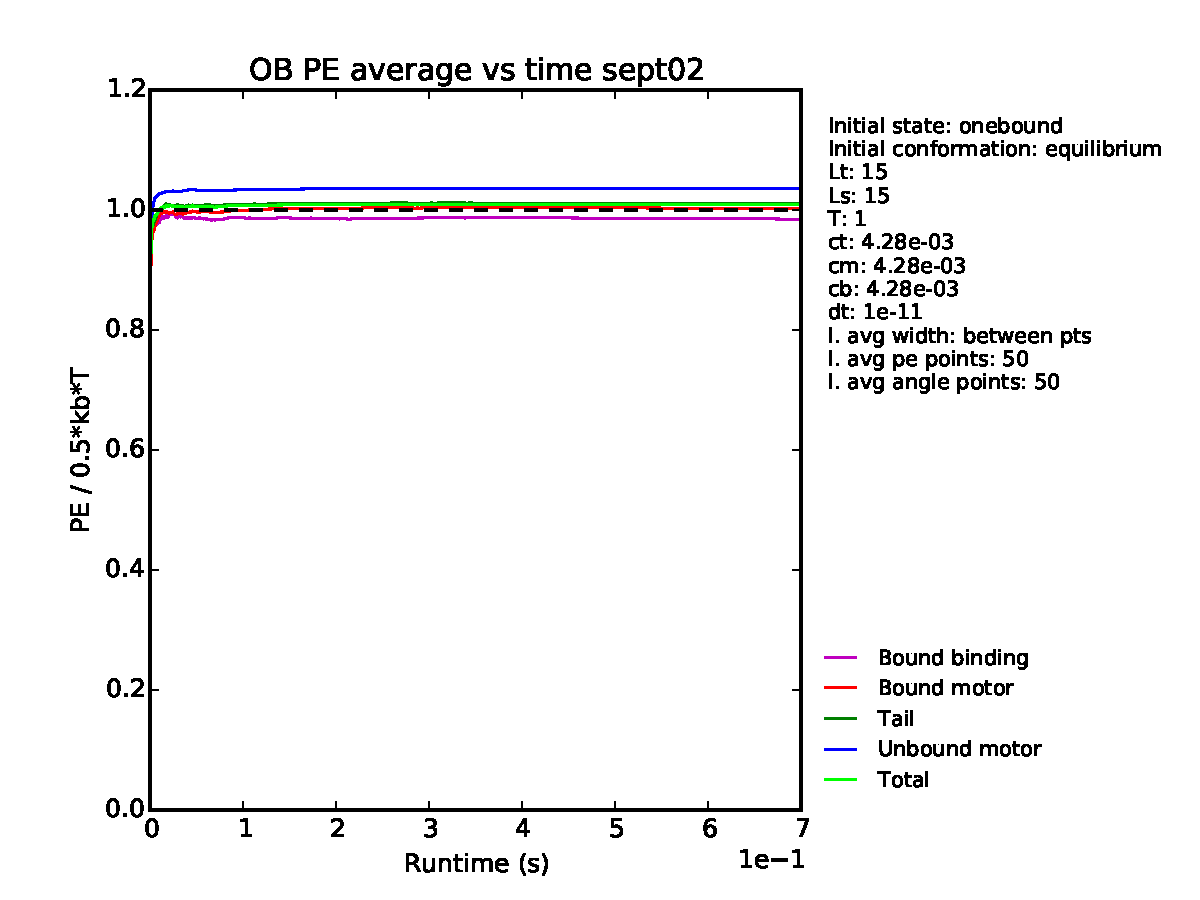
\includegraphics[width=\textwidth]{../figures/OB_Average_PE.pdf}
    \caption{Onebound PE vs time.}
  \end{minipage}
  \begin{minipage}[b]{0.49\textwidth}
    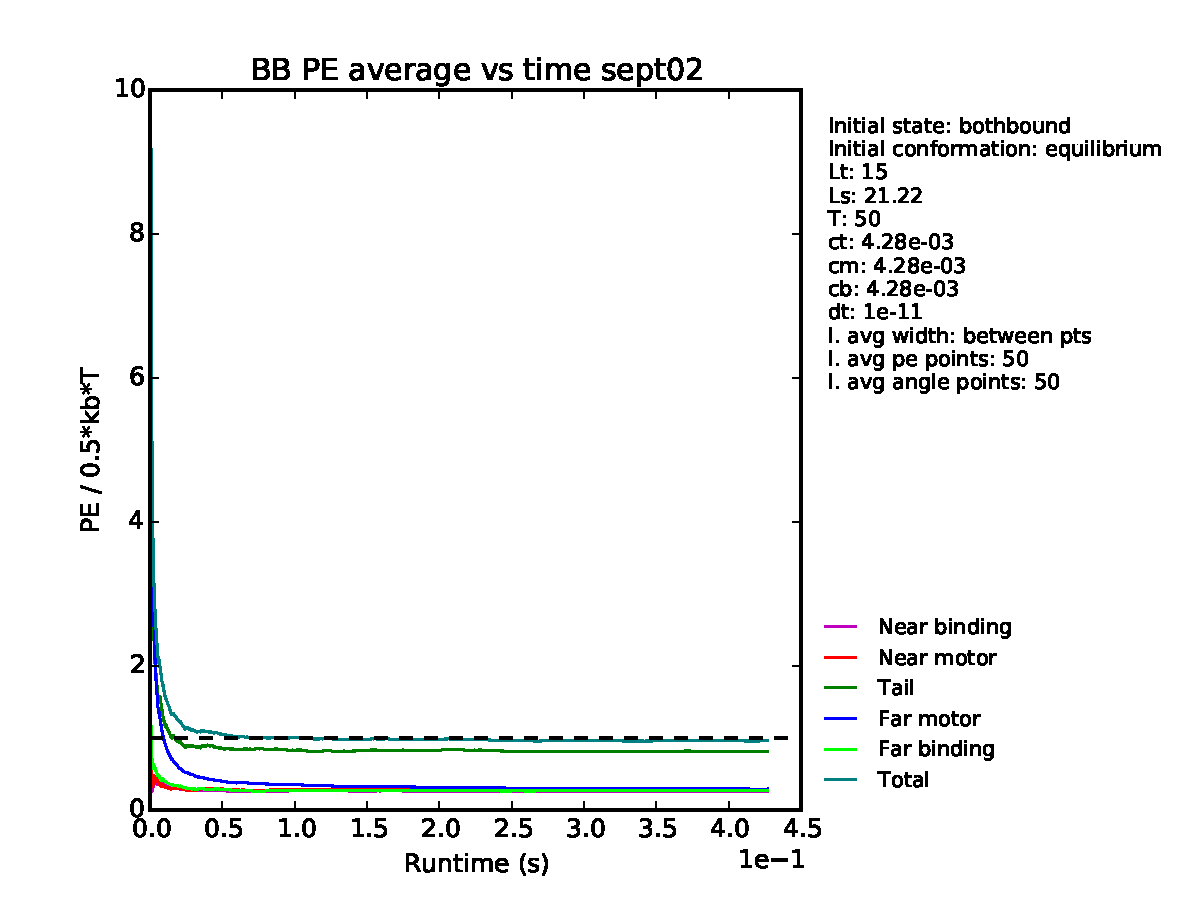
\includegraphics[width=\textwidth]{../figures/BB_Average_PE.pdf}
    \caption{Bothbound PE vs time.}
  \end{minipage}
  \label{fig:equipartition_agreement}
\end{figure}

\section{Physical Parameters}

\begin{figure}
  \centering
  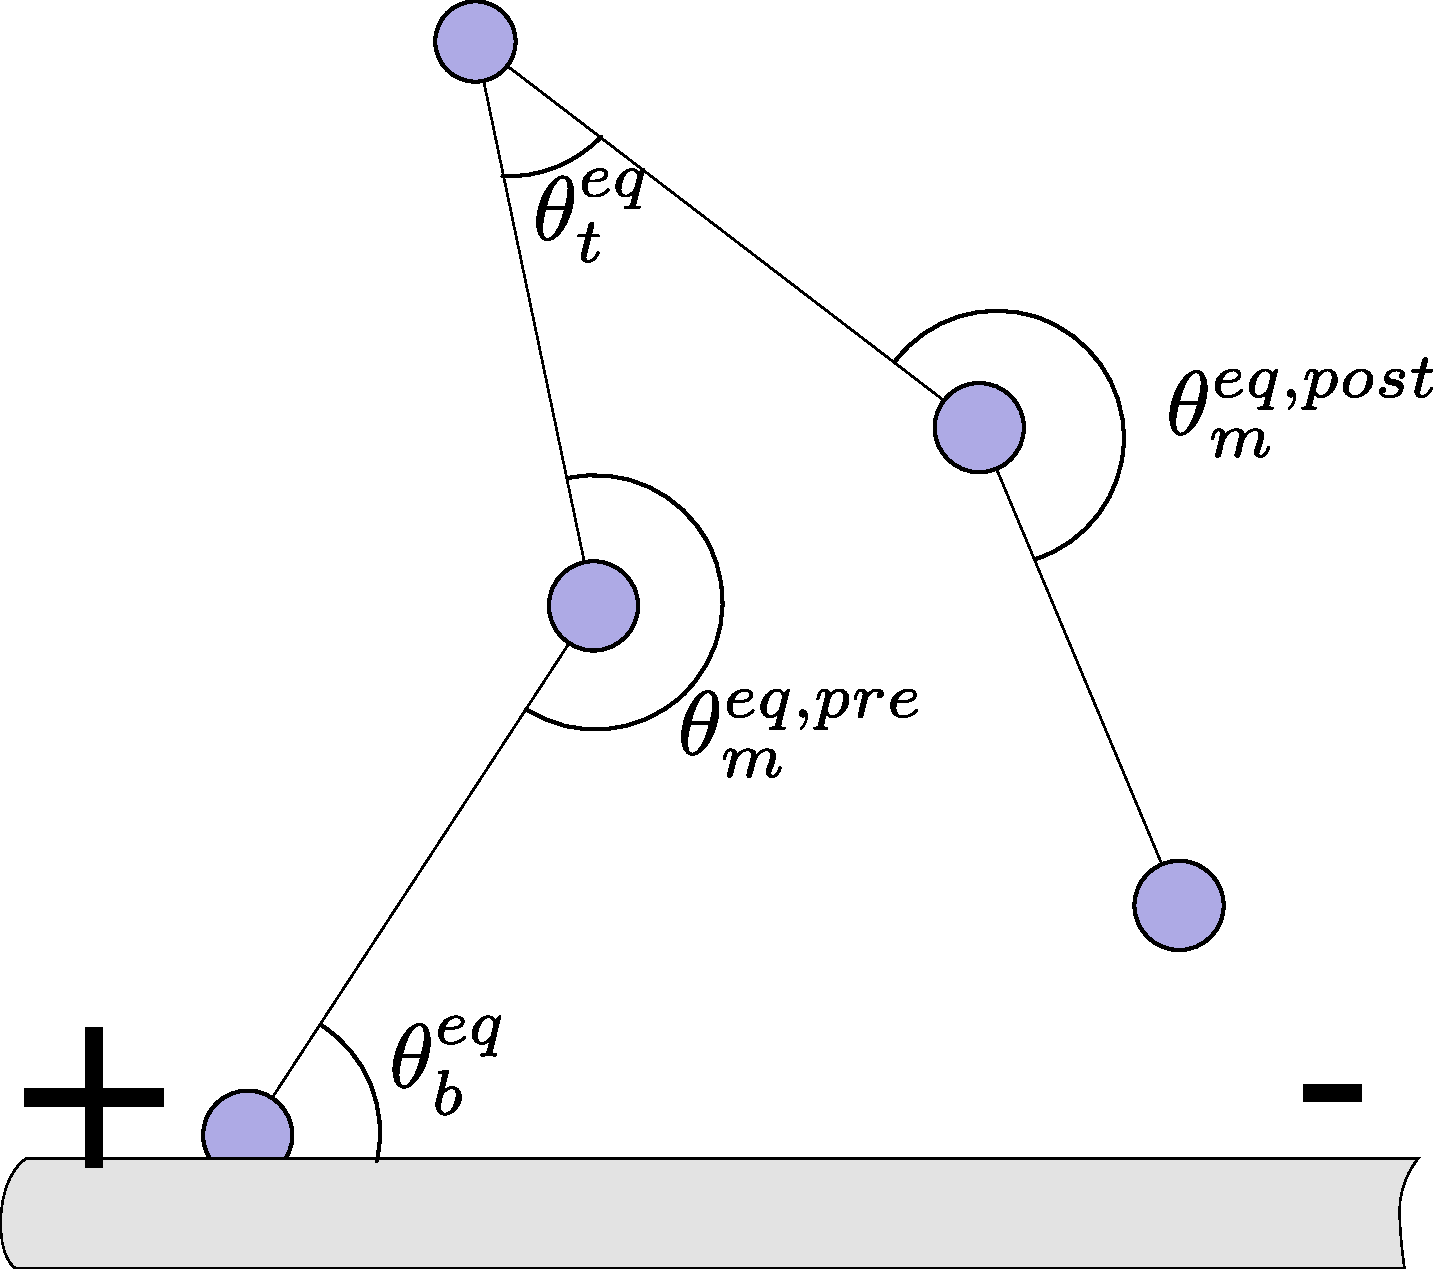
\includegraphics[width=.45\textwidth]{../figures/equilibrium-onebound}
  \caption{Definition of equilibrium angles.}
  \label{fig:eq_angles}
\end{figure}

\begin{center}
  \begin{tabular}{| l | l | l | l | l | l | l | l | l |}
    \hline
    & Winch (Sarlah) & Schmidt & Lin & PyMol 3VKH & PyMol 4RH7 & Redwine & Kon & Burgess \\\hline
    $L_s$ & 12nm & & & 21.0nm & 22.1nm & & & \\ \hline
    $L_t$ &  7nm & & & & 11.15nm & & & \\ \hline
    $R_b$ &  & & & 1.57nm & 1.45nm & & & \\ \hline
    $R_m$ &  7nm & & & 7.36nm & 6.3nm & & & \\ \hline
    $R_t$ &  & & & & 2.16nm & & & \\ \hline
    $\theta_{m}^{Pre}$ & 250$^{\circ}$ & & 171$^{\circ}$ & & & & & 160\\ \hline
    $\theta_{m}^{Post}$ & 330$^{\circ}$ & & 137.5$^{\circ}$ & & & & & 136\\ \hline
    $\theta_{b}$ & 56$^{\circ}$ & & 63.5$^{\circ}$ & & & & & \\ \hline
    $\theta_{t}$ & 0$^{\circ}$ & & & & & & & \\ \hline
    $k_{ub}$ & $180 s^{-1,a}$ & & & & & & $90.2 \pm 4.5$& \\ \hline
    $k_b$ & $5000 s^{-1,b}$ & & & & & & & \\ \hline
    $\Delta G_{bind, bb}$ & & & & & & -71 kJ/mol & & \\ \hline
    $\Delta G_{bind, ob}$ & & & & & & -37 kJ/mol & & \\ \hline
    $c_t$ & & & & & & & & \\ \hline
    $c_m$ & & & & & & & & \\ \hline
    $c_b$ & & & & & & 140 kJ/mol & & \\ \hline
  \end{tabular}
\end{center}

---- not sure if the Lin angles are right, since measuring the angle that the tail makes is \textit{not} necessarily the angle the angle the linker makes ----\\

a: Sarlah \textit{et al} gives us two different rate constants which could represent the bothbound to onebound transition: motor dissociation from the microtubule ($k_{-MT} = 460 s^{-1}$) and ATP hydrolysis/taking on the prestroke conformation ($k_{RS} = 180 s^{-1}$). We take the rate-limiting step $k_{RS}$ as our transition rate from bothbound to onebound since it is the slower of the two.\\

b: There are several Sarlah \textit{et al} rate constants we could use for the onebound to bothbound rate constant: binding to the microtubule ($k_{+MT} = 10^4 s^{-1}$), releasing a phosphate from hydrolysis ($k_{-Pi} = 5000 s^{-1}$) or the power stroke itself ($k_{PS} = 5000 s^{-1}$). We choose to represent the transition with $k_{-Pi} = 5000 s^{-1}$ because all these rates are fairly similar. We do not want to use the MT-binding rate because it could include both binding kinetics as well as MT-search kinetics, the latter of which we do not want to include in our binding rate.\\

\subsection{Stalk and tail length}
Sarlah et. al use stalk and tail lengths of 12 and 14 nm, respectively. We used PyMol to examine the crystal structures 3VKH and 4RH7 (pre and post-powerstroke) to find these values. The linker is roughly residues 1250-1510, calculated by eye.\\

\subsection{Finding Arrhenius preexpontential from k}
Papers often supply rate constants for various transitions. Our model uses Arhennius-type rates which take into account the change in conformational energy from switching equilibrium angles, so we must convert between free energy and rates:

\begin{align*}
  k_{bind} &= Ae^{-\beta(\Delta G_{bind} + \Delta G_{conf})}\\
  k_{bind} &= \left(Ae^{-\beta\Delta G_{bind}}\right)e^{-\beta\Delta G_{conf}}\\
  k_{bind} &= Be^{-\beta\Delta G_{conf})}\hspace{2cm}\mbox{B constant at constant T}\\
  \left<k_{bind}\right> &= \left<Be^{-\beta\Delta G_{conf}}\right>\\
  \left<k_{bind}\right> &= Be^{-\beta\Delta \left<G_{conf}\right>}\\
  \left<\Delta G_{conf}\right> &= \frac{1}{2}k_BT = \frac12\beta^{-1}\hspace{2cm}\mbox{David, what was the justification for this again?}\\
  \left<k_{bind}\right> &= Be^{-1/2}\\
  \rightarrow B &= k_{bind}\sqrt{e}
\end{align*}

\subsection{Properly implementing binding rates}
To determine if it is time to do a state transition, we calculate the per-timestep
transition probability $k_b/dt$, pick a number between zero and one, and transition
if our number was the lower of the two.\\

One issue with this is the rate constant $k_b$ is calculated experimentally from an
ensemble of dynein, and doesn't take into account how transitions are much more likely in some orientations than others. In reality, dynein will only bind to the MT when
its binding domain is less than 0.2nm away from a binding site.\\

To fix this, we define a parameter $n$, the time fraction onebound dynein is capable
of binding. Then a weighted average of the bindable and non-bindable rate constants
looks like:

\begin{equation*}
  nk_{bindable} + (n-1)k_{nonbindable} = k_b
\end{equation*}

Since we say $k_{nonbindable} = 0$, $k_{bindable}$, our effective rate constant of
binding, is $k_b/n$. Thus our preexponential Arrenhius factor is (see above):

\begin{equation*}
  B = \frac{k_{b}\sqrt{e}}{n}
\end{equation*}

\subsubsection{Calculating $n$}
A script, \verb|simulations/get_binding_time_fraction.py|, calculates how often
a onebound dynein spends in a bindable state:

\verbatiminput{../simulations/simulation_results/binding_time_fraction.txt}

\subsection{Calculating $\Delta G_{bind}$}
Based on Van der Spoel \textit{et. al.}, $\Delta H_{HB} = 10.6kJ/mol$ for water molecules forming a single hydrogen bond. Based on another paper (Anderson \textit{et al}), the
``stabilizing energy'' of a single salt bridge (H-bond between charged molecules) is about 16 kJ/mol.\\

Based on the interpreted bonds from crystal structures of the MTBD-MT complex shown in Redwine \textit{et. al}, there are 5.9 salt bridges in the high-affinity MTBD-MT
complex and 3.1 in the low-affinity complex. Thus if we guess the free energy of a salt bridge as 12 kJ/mol, we can estimate binding energies as:

\begin{align*}
  \Delta G_{bind, high-affinity} &= -71 \mbox{ kJ/mol}\\
  \Delta G_{bind, low-affinity} &= -37 \mbox{ kJ/mol}\\
\end{align*}

\subsection{Estimating $c_b$ spring constant}
If the energy of binding of the MTBD foot to the MT is -71 kJ/mol, we can get a rough estimate of the spring constant for the binding domain. We say that
$\Delta \theta \approx 0$ corresponds to being fully bound and $\Delta \theta \approx 1$ corresponds to breaking all salt bridges and being unbound. Thus:

\begin{align*}
  \frac 12 c_b \Delta \theta_{ba}^2 = \Delta G_{bind, high} &\rightarrow c_b = 2\Delta G_{bind, high} \approx 140 \mbox{ kJ/mol}\\
\end{align*}

\subsection{ATP Concentration from Weihong's Paper}
Weihong says in the Supplemental Methods section that the ATP concentration of the ``dynein motility buffer'' used to take his videos was 1mM, with no added ADP or Pi.\\

\subsection{Parameter hunt}
Lots of different manual simulations and their outcomes.

\begin{center}
  \begin{tabular}{| l | l | l | l | l | l | l | p{3cm} | p{2cm} | p{5cm} |}
    \hline
    Ls & Lt & kb & kub & cm & cb & ct & $\Big<P(\mbox{unbind per dt})\Big>$ & $\Big<\mbox{step time}\Big>$ & errors\\\hline
    22.1 & 11.1 & 5000 & 5000 & 0.02 & 0.02 & 0.02 & NA      & NA     & keeled over after ns\\\hline
    22.1 & 11.1 & 5000 & 5000 & 0.11 & 0.11 & 0.11 & $9e-9 $ & 1.7e-4 & keeled over after ns\\\hline
    22.1 & 11.1 & 5000 & 5000 & 0.18 & 0.18 & 0.18 & $4e-9 $ & 3.4e-4 & no error yet\\\hline
    22.1 & 11.1 & 5000 & 5000 & 0.23 & 0.23 & 0.23 & $3e-9 $ & 2.9e-4 & no error yet\\\hline
    22.1 & 11.1 & 5000 & 5000 & 0.58 & 0.58 & 0.58 & $2e-10$ & 3.3e-4 & no error yet\\\hline
    22.1 & 11.1 & 5000 & 3500 & 1.00 & 1.00 & 1.00 & ?? & 6.8e-4 & no error yet\\\hline
    22.1 & 11.1 & 5000 & 2000 & 1.00 & 1.00 & 1.00 & ?? & 1.6e-3 & weirdly stepped so L is around zero (0.04), maybe write a nudge to prevent this?\\\hline
    22.1 & 11.1 & 5000 & 1000 & 1.00 & 1.00 & 1.00 & ?? & 1.9e-3 & weirdly stepped so L is around zero (0.04), maybe write a nudge to prevent this?\\\hline
    22.1 & 11.1 & 5000 &  100 & 1.00 & 1.00 & 1.00 & ?? & 7.9e-3 & no error yet\\\hline
    22.1 & 11.1 & 5000 & 5000 & 1.16 & 1.16 & 1.16 & $6e-12$ & 8.4e-4 & no error yet\\\hline
    22.1 & 11.1 & 5000 & 5000 & 1.74 & 1.74 & 1.74 & $1e-13$ & 3.3e-3 & no error yet\\\hline
    22.1 & 11.1 & 5000 & 5000 & 2.32 & 2.32 & 2.32 & $7e-16$ & 9.0e-3 & no error yet\\\hline
    22.1 & 11.1 & 5000 & 3500 & 2.32 & 2.32 & 2.32 & ?? & 1.3e-2 & no error yet\\\hline
    22.1 & 11.1 & 5000 & 2000 & 2.32 & 2.32 & 2.32 & ?? & 1.3e-2 & no error yet\\\hline
    22.1 & 11.1 & 5000 & 1000 & 2.32 & 2.32 & 2.32 & ?? & 4.6e-2 & no error yet\\\hline
    22.1 & 11.1 & 5000 &  100 & 2.32 & 2.32 & 2.32 & ?? & ?? & no error yet\\\hline
    22.1 & 11.1 & 5000 & 5000 & 2.90 & 2.90 & 2.90 & $2e-18$ & 7.2e-2 & no error yet\\\hline
    22.1 & 11.1 & 5000 & 5000 & 3.49 & 3.49 & 3.49 & $5e-21$ & ?? & no error yet\\\hline
  \end{tabular}
  \textbf{Old probably wrong angle scheme run data}
\end{center}

\begin{center}
  \begin{tabular}{| l | l | l | l | l | l | l | p{3cm} | p{2cm} | l | p{5cm} |}
    \hline
    Ls & Lt & kb & kub & cm & cb & ct & $\Big<P(\mbox{unbind per dt})\Big>$ & $\Big<\mbox{step time}\Big>$ & run & errors\\\hline
    22.1 & 11.1 & 5000 & 5000 & 0.02 & 0.02 & 0.02 & & & & NaN! tail crashes into MT \\\hline
    22.1 & 11.1 & 5000 & 5000 & 0.11 & 0.11 & 0.11 & & & & NaN! motor crashes into MT \\\hline
    22.1 & 11.1 & 5000 & 5000 & 0.18 & 0.18 & 0.18 & & & & NaN! tail crashes into MT \\\hline
    22.1 & 11.1 & 5000 & 5000 & 0.23 & 0.23 & 0.23 & & $3.7e-4$ & & NaN! tail crashes into MT \\\hline
    22.1 & 11.1 & 5000 & 5000 & 0.58 & 0.58 & 0.58 & & $9.1e-4$ & & NaN! motor crashes into MT \\\hline
    22.1 & 11.1 & 5000 & 5000 & 1.16 & 1.16 & 1.16 & $2.7e-13$ & $6.8e-4$ & & \\\hline
    22.1 & 11.1 & 5000 & 5000 & 1.74 & 1.74 & 1.74 & & & & \\\hline
    22.1 & 11.1 & 5000 & 5000 & 2.32 & 2.32 & 2.32 & & & & \\\hline
    22.1 & 11.1 & 5000 & 5000 & 2.90 & 2.90 & 2.90 & $9.5e-32$ & & & \\\hline
    22.1 & 11.1 & 5000 & 5000 & 3.49 & 3.49 & 3.49 & $2.7e-35$ & & & \\\hline
    22.1 & 11.1 & 5000 & 3500 & 1.00 & 1.00 & 1.00 & $2.7e-12$ & $1.7e-3$ & & NaN! motor crashes into MT\\\hline
    22.1 & 11.1 & 5000 & 3500 & 2.32 & 2.32 & 2.32 & $4.1e-18$ & $5.5e-3$ & & \\\hline
    22.1 & 11.1 & 5000 & 2000 & 1.00 & 1.00 & 1.00 & $1.5e-12$ & $2.2e-4$ & & \\\hline
    22.1 & 11.1 & 5000 & 2000 & 2.32 & 2.32 & 2.32 & $2.2e-18$ & & & \\\hline
    22.1 & 11.1 & 5000 & 1000 & 1.00 & 1.00 & 1.00 & & & & \\\hline
    22.1 & 11.1 & 5000 & 1000 & 2.32 & 2.32 & 2.32 & & & & \\\hline
    22.1 & 11.1 & 5000 &  180 & 1.00 & 1.00 & 1.00 & & $1.8^{-2}$ & & \\\hline
    22.1 & 11.1 & 5000 &  180 & 1.30 & 1.30 & 1.30 & & $1.9^{-2}$ & & \\\hline
    22.1 & 11.1 & 5000 &  180 & 1.60 & 1.60 & 1.60 & & $1.9^{-2}$ & & \\\hline
    22.1 & 11.1 & 5000 &  180 & 1.90 & 1.90 & 1.90 & & $1.9^{-2}$ & & \\\hline
    22.1 & 11.1 & 5000 &  180 & 2.10 & 2.10 & 2.10 & & $1.9^{-2}$ & & \\\hline
    22.1 & 11.1 & 5000 &  180 & 2.25 & 2.25 & 2.25 & & $1.9^{-2}$ & & \\\hline
    22.1 & 11.1 & 5000 &  180 & 2.40 & 2.40 & 2.40 & & $1.9^{-2}$ & & \\\hline
    22.1 & 11.1 & 5000 &  180 & 2.55 & 2.55 & 2.55 & & $1.9^{-2}$ & & \\\hline
    22.1 & 11.1 & 5000 &  180 & 2.70 & 2.70 & 2.70 & & $1.9^{-2}$ & & \\\hline
    22.1 & 11.1 & 5000 &  180 & 3.10 & 3.10 & 3.10 & & $1.9^{-2}$ & & \\\hline
  \end{tabular}
  \textbf{New possibly right angle scheme run data}
\end{center}

ARE THESE ANGLES RIGHT??????????????\\

If the mean stepping rate from Weihong's paper is about 1 step / .1 seconds, then at a dt of $1e-11$s would lead to a desired unbinding
probability of $1e-11s/.1s = 1e-10$. The stepping probability was determined by printing out a random subset of unbinding probabilities
for the bothbound case, then averaging.\\

A more reliable step time determiner is $\Big<\mbox{step time}\Big>$, which should be around 0.1. This number can be determined from our step time histograms.\\

\section{Papers}

\subsection{Interesting Crystal Structures}
\textbf{3VKH} 2.8A x-ray resolution full dynein motor, from Kon 2012 (2.8A crystal structure of the dynein motor domain). Probably what we'll use to get some equilibrium angles and lengths, though not sure if crystal structures are identical to in vivo structures. Discusses amino acid chemistry of the powerstroke and long-distance MTBD/ATPase communication.\\
\textbf{3J67/3J68} 34A EM structure of pre/post motor (from Structural Mechanism of dynein power stroke 2014). Shows in-depth changes to motor, but appears to only be the six ATPases and possibly buttress.
\textbf{3J1T/3J1U} 9.7A EM structure of tightly/loosly bound tubulin-MTBD binding from (Structural basis for microtubule binding and release by dynein).\\
\textbf{4RH7} 2.3A x-ray crystal structure of dynein motor/stalk with ADP.Vi (pre-stroke) from (Structure of human cytoplasmic dynein-2 primed for its power stroke). Could be another good place to get angles for pre-stroke, since 3VKH is post-stroke.\\

\subsection{H-bond $\Delta G$ calculation paper}
van der Spoel, D., J. van Maaren, P., Larsson, P., Timneanu, N. ``Thermodynamics of Hydrogen Bonding in Hydrophilic and Hydrophobic Media'' \textit{J. Phys. Chem. B} 2006: 110, 4393-4398.\\

This paper uses classical simulations of water and alcohols to calculate thermodynamic parameters for the transition state and equilibrium state of water-water and water-alcohol
hydrogen bonds. It uses H-bond lifetime and the Eyring rate equation to calculate transition state $\Delta G$ and number of H bond pairs / unbonded pairs to find equilibrium
$\Delta G$. It then uses a Van't Hoff calculation to find enthalpies and entropies. Raman spectroscopy is shown to find a different enthalpy for water-water H-bonds. Findings:

\begin{center}
  \begin{tabular}{| l | l | l | l | l | l |}
    \hline
    & $\Delta G$ & $\Delta H$ & $T\Delta S$ \\\hline
    Simulation & 5.11 kJ/mol & 9.0 kJ/mol & 4.1 kJ/mol\\ \hline
    Experimental & 10.6 kJ/mol & & \\ \hline
  \end{tabular}
\end{center}

where T = 298.15K.\\

Another study (pH-Induced denaturation of proteins: a single salt bridge contributes 3-5 kcal/mol to the free energy of folding of T4 lysozyme by D. Anderson) found that
a single salt bridge contributes about 16 kJ/mol to stabilizing a protein. We can use these numbers as estimates of the binding energy of the motor.\\

\subsection{MTBD-Tubulin complex}
Redwine, W.B. \textit{et. al.} ``Structural basis for microtubule binding and release by dynein. '' Science 2012, 337(6101): 1532–1536.

This is a sub-nanometer MTBD-tubulin complex structure which shows how the complex forms. A cryo-EM structure was acquired, atomic-resolution structures for the high-affinity
MTBD and tubulin dimers were superimposed.  Rigid body docking and molecular dynamics was then used to optimize this structure. Another technique was used to figure out how
the low-affinity MTBD would bind, and yet another technique was used to translate between the low and high-affinity MTBDs to make an animation. Also did this with the Kon
vanadium onebound crystal structure and not much changed.\\

The MTBD-tubulin dimers are on the PDB as 3J1T for the high-affinity and 3J1U for the low-affinity structures.\\

After finding the high- and low-affinity structures for the complexes, the authors guess at what salt bridges form in the two states between MT and MTBD. The reported values are shown in the tables below.\\

\begin{table}
  \parbox{.45\linewidth}{
    \centering
    \begin{tabular}{| l | l |}
      \hline
      Residue & Occupancy \\\hline
      R3382-αE417 & 23\% \\\hline
      R3382-αE420 & 79\% \\\hline
      R3382-αG416 & 40\% \\\hline
      K3299-βE431 & 60\% \\\hline
      K3299-βD427 & 53\% \\\hline
      R3342-βE159 & 51\% \\\hline
      N3310-αG410 & 38\% \\\hline
      L3385-αE415 & 48\% \\\hline
      S3384-αG415 & 27\% \\\hline
      A3383-αE415 & 49\% \\\hline
      R3306-βE196 & 86\%*\\\hline
      R3337-βD199 & 2\%* \\\hline
      R3342-βN197 & 36\%*\\\hline
    \end{tabular}
    \caption{High-affinity MTBD-MT complex salt bridges. RH column is bonds between MTBD and MT, respectively.}
  }
  \hfill
  \parbox{.45\linewidth}{
    \centering
    \begin{tabular}{| l | l |}
      \hline
      Residue & Occupancy \\\hline
      A3383-αE415  & 45\% \\ \hline
      R3382-αG416  & 44\% \\ \hline
      R3382-αE417  & 61\% \\ \hline
      R3382-αE420  & 79\% \\ \hline
      K3299-βE196  & 27\% \\ \hline
      S3307-βR253  & 16\% \\ \hline
      L3385-αE415  & 34\% \\ \hline
      N3310-αK112  & 10\% \\ \hline
    \end{tabular}
    \caption{Low-affinity MTBD-MT complex salt bridges. RH column is bonds between MTBD and MT, respectively.}
  }
\end{table}

From this table we count the number of effective salt bridges in the high/low affinity complexes: 5.9 and 3.1, respectively.\\

Some \textbf{really} cool videos of the MTBD switching from high/low affinity states. If you could get a similar video of the AAA domains binding ATP, these would be really
cool videos to put in a presentation.\\

\subsection{Winch Model (dx.doi.org/10.1016/j.bpj.2014.06.022)}
-Communication between motors and BDs possible through $\alpha$-helix sliding. Bidirectional communication. [24,25]\\
-Pre, post-powerstroke states\\
-Pre-powerstroke: unbound state after ATP hydrolysis (our onebound)\\
-Post-powerstroke: bound state (our bothbound)\\
-Elastic stalk, unlike our rigid one\\
-Only tail angle changes between pre and post-powerstroke\\
-MTBD decides directionality?\\
-Tail-tail interaction, also motor-motor stacking interaction\\
-rate constant simulation, does not do dynamics to take into account time spent in a state\\

\textbf{Physical Parameters from Winch Model paper}:\\
Sarlah et al. use the following physical parameters for Dynein: $L_s = 12$nm binding angle: 34 degrees from vertical, motor
domain radius: 7nm. Their angle scheme is different than ours in that it has the linker/tail facing towards the MT, which looks different
from our facing-up tail. This might be a confusion on our part in the difference between the linker and the tail, but it may not. By assuming the linker starts at the top of the head and points downwards, we can calculate an estimate for tail length as $L_t = 7nm$.

\subsection{Annual Review, 8-state Mechanochemical diagram}
Cianfrocco, M*., DeSantis, M*., Leschziner, A., Reck-Peterson, S. ``Mechanism and Regulation of Cytoplasmic Dynein'' \textit{Annu. Rev. Cell. Dev. Biol.} 2015: 31:83-108.\\

Goes over in detail the various steps of the Dynein chemical cycle. Eight-state model as follows:\\

\begin{enumerate}
\item Dynein begins cycle with AAA1 binding site open.
\item ATP then binds to the AAA1 binding site.
\item ATP binding causes ``ring closure,'' where the AAA1 and AAA2 subdomains shift closer together.
\item Ring closure (ie ATP binding) causes the buttress to shift, causing the MTBD to lose MT affinity.
\item Ring closure (ATP binding) also causes the linker to bend 90 degrees, causing the monomer to enter the pre-powerstroke state. The order of states 4. and 5. is unknown, but entering pre-powerstroke \textit{after} unbinding from the MT causes more directional motion. The role of ATP hydrolysis also is not understood as of this paper (2015).
\item Random walk of the low-MT-affinity MTBD eventually leads to weak rebinding at a new place on the MT.
\item Rebinding causes a change in the MTBD back to its high affinity state. AAA4 moves to prevent steric clash when the linker straightens. AAA5/6 move away from AAA1 and the linker straightens to its post-powerstroke conformation. NOTE: this is distinct from the conformation in steps 1-4 in that AAA1/2 is still closed.
\item The linker shifts some more and AAA1/2 opens up, releasing ADP.
\end{enumerate}

\subsection{Weihong's Dynein stepping data}
Qiu, W., Derr, N., Goodman, B., Villa, E., Wu, D., Shih, W., Reck-Pterson, S. ``Dynein achieves processive motion using both stochastic and coordinated stepping.'' \textit{Nature Structural \& Molecular Biology}. 2012, 19:193-200.\\

Has the stepping histograms we are trying to reproduce computationally.

\subsection{Pre-powerstroke structure, linker remodel details}
Schmidt, H*., Zalyte, R*., Urnavicius, L., Carter, AP. ``Structure of human cytoplasmic dynein-2 primed for its power stroke.'' \textit{Nature} 2014. 518:435-438.

Describes how ATP hydrolysis ``closes the ring,'' sterically interacting with the linker to cause the pre-powerstroke conformation. Does so by presenting the crystal structure of Dynein AAA1-ADP.Vanadate. Goes over AAs responsible for nucleotide binding. Supplemental video of AAA1L-AAA2L gap closing in response to nucleotide-Vi binding. Supplemental video of linker swinging in response to ring closure. AAA2-4 system acts rigidly during the cycle. Discusses how steric clash is what makes the linker take on a 90-degree bent shape when the ring closes. Figure on Dynein-ADP buttress having no kink, whereas Dynein-ADP.Vi having a kink. The kink presumably changes MTDB binding affinity.

\subsection{3D Pre/Post-PS structures, there are two Pre-PS states!}
Jianfeng Lin, Kyoko Okada, Milen Raytchev, Maria C. Smith \& Daniela Nicastro. ``Structural mechanism of the dynein power stroke.'' \textit{Nature Cell Biology} 2014. 16:479-485.

This paper finds the 3D structures of both pre (3J68) and post (3J67)-powerstroke dynein. This paper is about \textbf{axonmenal} dynein, which seems to be wildly different from cytoplasmic dynein, but this paper doesn't really mention any differences. The paper claims there are three conformational states: prestroke-1 immediately after MT unbinding, prestroke-2 after MT-binding, then poststroke after the powerstroke. This paper claims that transitioning between the post and pre-powerstroke ``resembled an opening jackknife with an angular amplitude of ~65$^{\circ}$ or ~50$^{\circ}$, depending on which axonemal dynein. It is unclear what this jackknife metaphor is referring to - the linker?. They make the claim that \textit{rotation of the head is the principle mechanism of Dynein powerstroke, not linker remodelling}. They seem to be claiming that the major thing differentiating the three states is the motor domain/head angle. It starts out facing the MT in post-stroke, then rotates away from the MT by 50-70 degrees into pre-1, then rotates towards the MT by 20 degrees to enter pre-2. Not entirely sure if it's all axonemal, since the PDB page for the structures says it's a cytoplasmic gene.\\

Figure~\ref{fig:em_tomography_eq_angles} shows different measurements
for equilibrium angles from the data in this paper.
\begin{figure}[h!]
  \centering
  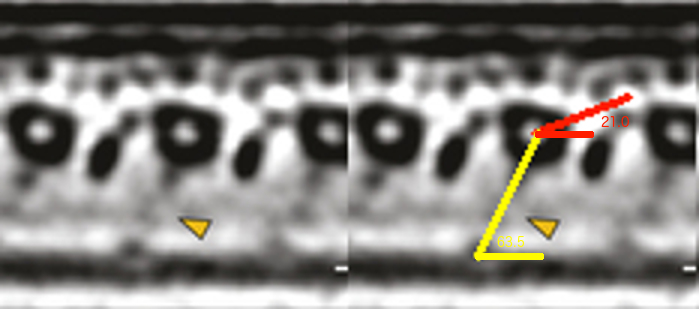
\includegraphics[width=.45\textwidth]{../figures/Post_powerstroke_tomography.jpg}
  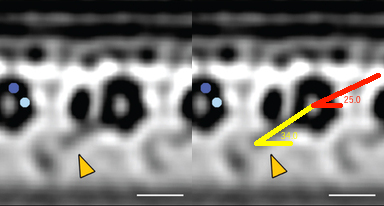
\includegraphics[width=.45\textwidth]{../figures/Pre_powerstroke_tomography.jpg}
  \caption{Post- and Pre-powerstroke equilibrium angles from EM tomography. Note: Ignore binding angle, the MTBD shouldn't actually be bound to MT.}
  \label{fig:em_tomography_eq_angles}
\end{figure}

\subsection{Linker position in Post-powerstroke dynein, two Post-PS states?}
Insights into dynein motor domain function from a 3.3A crystal structure, Hugo Schmidt, Andrew P. Carter\\

A crystal structure of just the motor domain in a low-ATP-affinity conformation. Suggests that differences between their structure and a Dictyostelium ADP-bound structure suggest there is a difference between AAA1 apo/ADP states, suggesting at least two post-powerstroke states. The paper postulates that linker interacting with AAA5 is what kicks out ADP. They say that linker-AAA5 complex creates a low-nucleotide-affinity state.\\

They further suggest that nucleotide binding causes the linker to unbind AAA5 and rebind AAA2 on nucleotide binding. Thus AAA5-linker is post-powerstroke apo and AAA2-linker is ATP-bound (pre or post powerstroke?)\\

ATPases 2, 3, 4 mutation leads to decreased velocity.\\

\subsection{Linker pre-powerstroke conformation}
ATP hydrolysis cycle-dependent tail motions in cytoplasmic dynein
Kon T, Sutoh K

This paper supposedly talks about how the linker changes conformation on ATP binding.\\

A FRET study on how ATP changes the distance of domains. They label the C-terminal tail and different regions on the motor, then calculate the FRET efficiency. FRETY efficiency is higher when ATP is present, indicating two different states based on ATP presence. They try to trap dynein in different states (apo, ATP, ADP-Pi, ADP) using different trapping nucleotide analogs. ADP-Vi dynein stayed in state II, while nonhydrolyzable ATP, apo, and ADP additions caused the motor to stay in state I.\\

The interpretation is that the dynein's tail moves from a state where it is near the C-terminus (AAA5) to one where it is near AAA2. 5->2 is prestroke on hydrolysis, 2->5 is poststroke on Pi rejection. ATP binding is what causes the conformation change, since they have trapped ATP-ish bound dyneins in both state I and II. The powerstroke happens during the ADP state, since they have an ADP-dynein in state II and another in state I.\\

They also report an ATPase $k_{cat} = 90.2 \pm 4.5$, meaning roughly 100 ATP are cycled per second.\\

\subsection{Possibly more equilibrium motor angles}
Dynein structure and power stroke
Nature 2003, Burgess and Oiwa

EM microscopy of apo/ADP-Vi flagellar dynein shows that the stem and stalk don't change length between two states, only the angle/position changes. The paper claims ``the origin of the movement is a displacement of the stem relative to the head and stalk.''.

Paper claims motor angle is \textbf{160 degrees in pre-stroke and 136 degrees in powerstroke}.\\

\textbf{Could we use the angle distribution histograms in \ref{fig:EM-angles-burgess} fit to a boltzmann factor with a spring energy to get cm?}

\begin{figure}[h!]
  \centering
  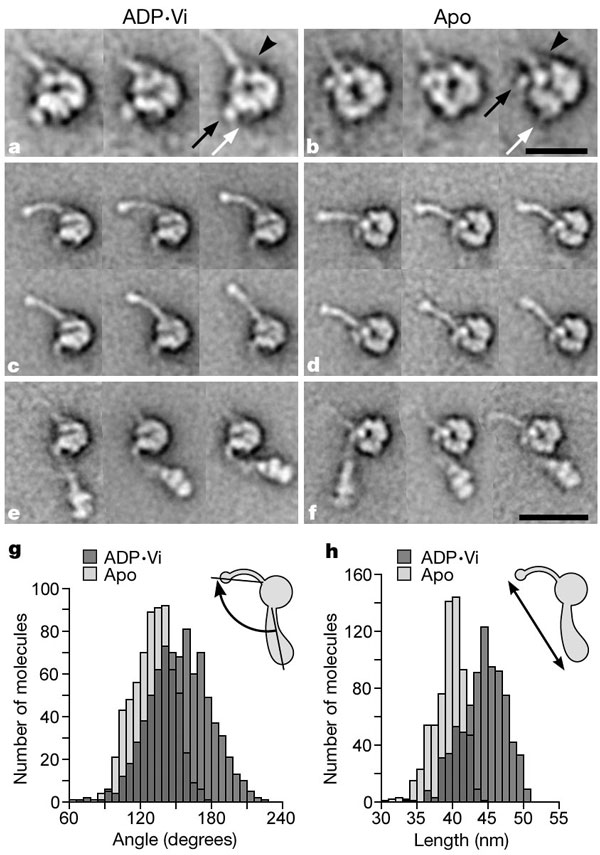
\includegraphics[width=.45\textwidth]{../figures/axonemal-motor-angles.jpg}
  \caption{Angle histograms from EM microscopy on axonemal (not cytoplasmic) dynein.}
  \label{fig:EM-angles-burgess}
\end{figure}


There is a difference in standard deviation of angles in pre/post-stroke. Pre-stroke has a stdev of 20 degrees, Post-stroke has a stdev of 11. The authors indicate this is due to stiffening of the stalk/foot domain. This seems like it would indicate changes in the motor spring constants between the pre/post-powerstroke states.

\subsection{2012 Kon Crystal Structure (3VKH)}
This paper crystallizes a full-length and MTBD-truncation mutants. 3VKH is the full-length, but one MTBD of the dimer did not come out in the crystal structure.

\subsection{Imamula Stepping Model}
This is an older (2007) paper presenting a chemical model and giving rate constants for MT un/binding. Averages are: $K_{d,pre} = 0.2uM$, $K_{d,post} > 10uM$. They determine these by adding a known concentration of monomeric Dynein apo, ATP, ADP-Pi or ADP, adding microtubules, removing MT-Dynein dimers and remeasuring concentration. These parameters are good in that equilibrium constants (as opposed to rate constants) \textit{don't} take into account kinetics, only free energy change...right?\\

Also, the paper says that axonemal dyneins have multiple motor domains, i.e aren't dimers, so that changes the results from the Lin paper. The binding angle is probably valid, though.\\

\subsection{Further reading}
\begin{itemize}
\item The dynein family at a glance. Höök P, Vallee RB J Cell Sci. 2006 Nov 1; 119(Pt 21):4369-71. The actual differences between axonemal/cytoplasmic dynein.
\end{itemize}

\section{Notes by David}
(This stuff can be deleted or edited or moved elsewhere...)

The mean speed of dynein is $134\pm 60$~nm~s$^{-1}$.  It looks like
perhaps the speed should be more like 80 or 80 nm/s~\cite{reck2006single}.

Its average step 1D displacement is 8~nm. (See page 194 of Weihong's \emph{Nature} paper.)

Together this means that the mean time between steps is about 60~ms.
Note milliseconds.  Thus we really need to be careful about how small
our $\Delta t$ is.

Note also another paper that is very similar to that of Weihong~\cite{dewitt2012cytoplasmic}.

\section{Program Scaling}
Program runtimes, as of commit 62c4d:

\begin{verbatim}
elliotc12@bennet:~/dynein_walk$ grep "dt" default_parameters.h 
double dt = 1e-11;
elliotc12@bennet:~/dynein_walk$ time ./generate_stepping_data --runtime=1e-5
Running for 1e-05 s

real	0m5.001s
user	0m4.972s
sys	0m0.000s
elliotc12@bennet:~/dynein_walk$ time ./generate_stepping_data --runtime=1e-5
Running for 1e-05 s

real	0m7.121s
user	0m7.072s
sys	0m0.000s
elliotc12@bennet:~/dynein_walk$ time ./generate_stepping_data --runtime=1e-4
Running for 0.0001 s

real	0m26.666s
user	0m26.608s
sys	0m0.000s
elliotc12@bennet:~/dynein_walk$ time ./generate_stepping_data --runtime=1e-4
Running for 0.0001 s

real	0m29.479s
user	0m29.428s
sys	0m0.000s
elliotc12@bennet:~/dynein_walk$ time ./generate_stepping_data --runtime=1e-3
Running for 0.001 s

real	4m47.224s
user	4m46.832s
sys	0m0.000s
elliotc12@bennet:~/dynein_walk$ time ./generate_stepping_data --runtime=1e-3
Running for 0.001 s

real	4m56.207s
user	4m55.776s
sys	0m0.000s
elliotc12@bennet:~/dynein_walk$ time ./generate_stepping_data --runtime=1e-2
Running for 0.01 s

real	61m44.302s
user	61m35.264s
sys	0m0.120s
\end{verbatim}

The average time per iteration is ~3.9 microseconds, or 3.9e5 real seconds per simulated second at $dt=10^{-11}s$. Thus we can generate one 60-millisecond step in 23,400 seconds, or 6.5 hours. A thousand-step simulation would thus take, very roughly, 8 months.\\

\section{Todo}
\begin{itemize}
\item Add dt testing figure to thesis\_stuff.tex.
\item Make all figures in thesis\_stuff.tex be dependencies of thesis\_stuff.tex in the Makefile; it should be deducible to a novice how every figure is generated in code.
\item Check out kinetic parameters papers in the Winch model, see how they are aquired
\item Generate a figure explaining how our model simplifies the rate constants in the Winch paper / annual review.
\item Make a figure with PyMol visualizations with and without our model superimposed
\item Calculate Dynein motor efficiency by finding friction work on cargo and energy of ATP.
\item Make Dynein binding rate diagram showing how our model relates to the Imamula one
\item Make pretty dynein visualization in PyMol (or some software) showing how dimerization happens AND how docking to the MT happens; ask David what this should look like
\end{itemize}

\bibliographystyle{plain}
\bibliography{thesis_stuff}

\end{document}
